\documentclass[../main.tex]{subfiles}
\begin{document}
	When pulse is so intense that it ionize the medium, this contribution
	follows the evolution equation for electron density.

	\begin{equation} \label{eq:electron}
		\frac{\partial \rho}{\partial t} =
		W_{MPI}(\mathcal{I})(\rho_{nt} - \rho) +
		W_{ava}(\mathcal{I})\rho
	\end{equation}
	Where $W_{MPI}$ is multiphoto ionization rate [eq:~\ref{eq:MPI_Rate}]
	and $W_{ava}$ is avalanche ionization rate. The avalanche ionization
	rate is proportional to the pulse intensity.
	\begin{equation} \label{eq:ava_rate}
		W_{ava}(\mathcal{I}) = \sigma(\omega_0) \frac{\mathcal{I}}{U_i}
	\end{equation}
	Where $\sigma(\omega_0)$ is the inverse Bremsstrahlung coefficient.
	We can describe avalanche rate as a current using same formalism
	as~[eq:~\ref{eq:eff_current}, \ref{eq:current}]
	Adding avalanche term and
	converting $(\zeta, \tau)$ to $(z,t)$ our NLS [eq:~\ref{eq:nls_abs}] becomes
	\begin{widetext}
	\begin{equation} \label{eq:nls_com}
		\frac{\partial \mathcal{E}}{\partial z}
		+ i\frac{\beta_2}{2} \frac{\partial^2 \mathcal{E}}{\partial t^2}
		- \frac{i}{2n_0k_0}\Delta_\perp \mathcal{E}
		= in_2k_0\mathcal{I} \mathcal{E}
		- \frac{\beta_K}{2}\mathcal{I}^{K-1} \mathcal{E}
		- \frac{\sigma(\omega)}{2}(1 + i\omega_0 \tau_c)\rho\mathcal{E}
	\end{equation}
	\end{widetext}


	The Nonlinear Schrödinger Equation in its  extended form
	[eq:~\ref{eq:nls_com}] represent pulse beam propagation through a
	transparent medium. Beam propagation mainly governed by second order
	dispersion (second term), diffraction (third term), optical Kerr effect
	(fourth term), photoionization and avalanche ionization (fifth and sixth
	term).

	While optical Kerr effect induced self focusing try to collapse laser
	beam, absorption and ionization induced plasma defocusing try to stop
	that.

	\begin{figure}[h] ~\cite{couairon_femtosecond_2007}
		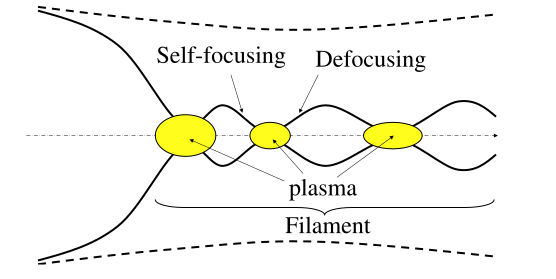
\includegraphics[width=0.5\textwidth]{images/filament.png}
	\caption{Schematic representation of the focusing–defocusing cycles undergone by the intense core of the beam. The solid curves indicate the diameter
of the intense core. The flamentation length is the distance covered by these cycles. The dashed line indicates the root mean square radius of the
full beam \label{fig:filament}}
	\end{figure}

	Figure [~\ref{fig:filament}] shows a cartoon of focusing-defocusing
	phenomenon. Laser beam of power above than critical power goes into self
	focusing and try to collapse. However when beam become sufficiently
	intense, MPA attenuate core of beam and plasma generation happen around
	the core of beam. This plasma defocus beam. Once defocused, laser beam
	can still have power higher than critical power therefore it can start
	to collapse again. This process keep repeating itself and flamentat can
	sustain for long distances without any external waveguide.

\end{document}
